%导演区
\documentclass[a4paper,11pt,UTF8]{article}%book,report,letter
\usepackage[table]{xcolor}
\usepackage{ctex}
\usepackage{geometry}
\geometry{a4paper,scale=0.8}
\usepackage{amsfonts}
\usepackage{amssymb}
\usepackage{verbatim}
\usepackage{mathrsfs}
\usepackage[arrow,matrix]{xy}
\usepackage{amsmath,amssymb,amscd,bm,bbm,amsthm,mathrsfs}
\usepackage{amsmath,amscd}
\usepackage{amsfonts,amssymb}
\usepackage{xypic}
\usepackage{indentfirst}
\usepackage{diagbox}
\usepackage{graphicx}
\usepackage{subfig}    %% 子图包
\usepackage{float} 
\usepackage{caption}
\captionsetup{labelfont=bf}
\usepackage{zhnumber} % change section number to chinese
%这下面为在latex中插入代码所需环境
\usepackage{CJK}
\usepackage{listings}
\usepackage{xcolor}
\lstset{
	language=Matlab,  %代码语言使用的是matlab
	frame=shadowbox, %把代码用带有阴影的框圈起来
	rulesepcolor=\color{red!20!green!20!blue!20},%代码块边框为淡青色
	keywordstyle=\color{blue!90}\bfseries, %代码关键字的颜色为蓝色,粗体
	commentstyle=\color{red!10!green!70}\textit,    % 设置代码注释的颜色
	showstringspaces=false,%不显示代码字符串中间的空格标记
	numbers=left, % 显示行号
	numberstyle=\tiny,    % 行号字体
	stringstyle=\ttfamily, % 代码字符串的特殊格式
	breaklines=true, %对过长的代码自动换行
	extendedchars=false,  %解决代码跨页时,章节标题,页眉等汉字不显示的问题
	texcl=true}
\def\d{\textup{d}}

\theoremstyle{plain}
\newtheorem{thm}{定理}[section]
\newtheorem{lem}{引理}[section]
\newtheorem{prop}{命题}[section]
\newtheorem{cor}{推论}[section]


\renewcommand{\qedsymbol}{$\square$}
\renewcommand\baselinestretch{1.25}
\renewcommand\thesection{\zhnum{section}}
\renewcommand \thesubsection {\arabic{section}}

\usepackage{tabu}                     % 表格插入
\usepackage{multirow}                 % 一般用以设计表格,将所行合并
\usepackage{multicol}                 % 合并多列
\usepackage{multirow}                % 合并多行
\usepackage{float}                    % 图片浮动
\usepackage{makecell}                 % 三线表-竖线
\usepackage{booktabs} 
%正文区
\begin{document}
	\title{\heiti 课题组组会-练习6}
	\author{王程 }
	\date{\today}
	\maketitle
	
	\section{练习及结果}
	1.在$x\in \left[0,1\right]$ 的均匀网格上尝试使用 Variational Reconstruction (VR) 对$f\left(x\right),g\left(x\right)$ 分别进行P0P2,P1P2重构,其中$f\left(x\right)=1+x+x^2,g\left(x\right)=sin\left(\pi x\right)$.\\
	\indent a)尝试调整不同阶次的权重系数及边界面权重系数,测试重构精度。\\
	\indent b)如果网格为不均匀网格呢?\\
	\indent c)如果考虑Hyperbolic rDG,进行DG(P0P2)+rDG(P0P1),使用VR重构算法,结果如何?\\
	~\\
	\noindent \textbf{a)解:P0P2}\\
\indent 本题均考虑非均匀网格,均匀网格视为非均匀网格的特例。\\
\indent 下面给出Interfacial jump integration 的定义以及P0P2的限制方程组。\\
$$I=\sum_{f=1}^{N_f}I_f, I_f=\frac{1}{d_{LR}}\left(\omega^2_0\left[u\right]^2+\omega^2_1\left[u_x\right]^2d^2_{LR}+\omega_2^2\left[u_{xx}\right]^2d^4_{LR}\right), \left[u\right]=u_L-u_R$$\\
限制方程组:
\\$$\left\{
\begin{aligned}
	\frac{\partial I_f}{\partial u_{2L}}&=0\\
    \frac{\partial I_f}{\partial u_{3L}}&=0\\
    \frac{\partial I_f}{\partial u_{2R}}&=0\\
    \frac{\partial I_f}{\partial u_{3R}}&=0
\end{aligned}
\right.$$

\noindent 即\\
\noindent $\left\{\small
\begin{aligned}
	&\frac{2}{d_{LR}}\left(\omega_0^2\left(\sum_{i=1}^{3}u_{iL}B_{iL}-\sum_{i=1}^{3}u_{iR}B_{iR}\right)B_{2L}+\omega_1^2\left(\frac{1}{\Delta x_{ieL}}\sum_{i=2}^{3}u_{iL}B_{i-1 L}-\frac{1}{\Delta x_{ieR}}\sum_{i=2}^{3}u_{iR}B_{i-1 R}\right)\frac{1}{\Delta x_{ieL}}d_{LR}^2\right)=0\\
	~\\
	&\frac{2}{d_{LR}}\left(\omega_0^2\left(\sum_{i=1}^{3}u_{iL}B_{iL}-\sum_{i=1}^{3}u_{iR}B_{iR}\right)B_{3L}+\omega_1^2\left(\frac{1}{\Delta x_{ieL}}\sum_{i=2}^{3}u_{iL}B_{i-1L}-\frac{1}{\Delta x_{ieR}}\sum_{i=2}^{3}u_{iR}B_{i-1 R}\right)B_{2L}\frac{1}{\Delta x_{ieL}}d_{LR}^2+\right.\\
	&\left.\omega_2^2\left(\Delta x_{ieL}^{-2}u_{3L}-\Delta x_{ieR}^{-2}u_{3R}\right)\Delta x_{ieL}^{-2} d_{LR}^4\right)=0\\
	~\\
	&\frac{-2}{d_{LR}}\left(\omega_0^2\left(\sum_{i=1}^{3}u_{iL}B_{iL}-\sum_{i=1}^{3}u_{iR}B_{iR}\right)B_{2R}+\omega_1^2\left(\frac{1}{\Delta x_{ieL}}\sum_{i=2}^{3}u_{iL}B_{i-1 L}-\frac{1}{\Delta x_{ieR}}\sum_{i=2}^{3}u_{iR}B_{i-1 R}\right)\frac{1}{\Delta x_{ieR}}d_{LR}^2\right)=0\\
	~\\
	&\frac{-2}{d_{LR}}\left(\omega_0^2\left(\sum_{i=1}^{3}u_{iL}B_{iL}-\sum_{i=1}^{3}u_{iR}B_{iR}\right)B_{3R}+\omega_1^2\left(\frac{1}{\Delta x_{ieL}}\sum_{i=2}^{3}u_{iL}B_{i-1L}-\frac{1}{\Delta x_{ieR}}\sum_{i=2}^{3}u_{iR}B_{i-1 R}\right)B_{2R}\frac{1}{\Delta x_{ieR}}d_{LR}^2+\right.\\
	&\left.\omega_2^2\left(\Delta x_{ieL}^{-2}u_{3L}-\Delta x_{ieR}^{-2}u_{3R}\right)\Delta x_{ieR}^{-2} d_{LR}^4\right)=0\\
\end{aligned}
\right.$\leavevmode\\
~\\
~\\
\indent 通过求解该线性方程组进行$f\left(x\right)$与$g\left(x\right)$的重构,需要注意的是,LU-SGS得到的解误差较大, 需要SGS(k)进行求解,且k=21。下面展示权重$\omega_0=1, \omega_1=1, \omega_2=1, \omega_b=\frac{\omega_0}{\sqrt{2}}$, Nelem=8时的重构图和精度分析图:\\
	\begin{figure}[!h]
	\centering
	\subfloat[f重构]{
		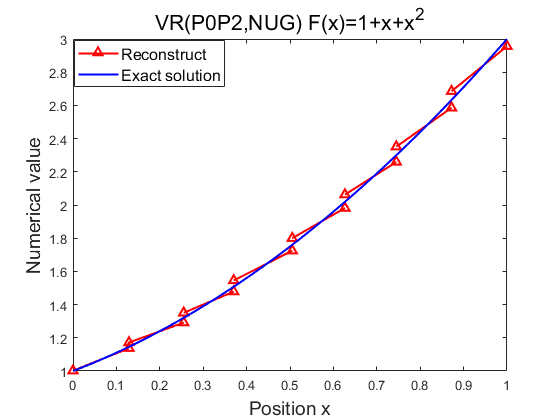
\includegraphics[width=3in]{P0P2VRreconstruct/Fu8LU-SGS.png} 
	}
	\hfill
	\subfloat[g重构]{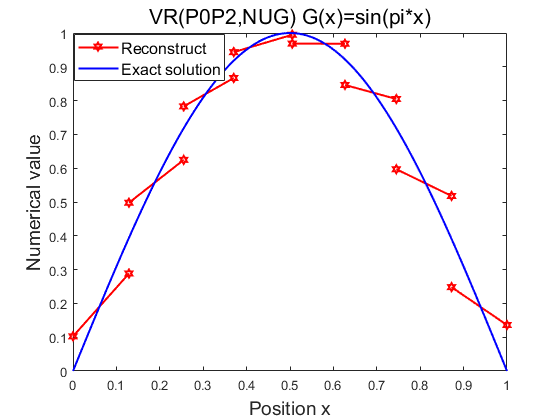
\includegraphics[width=3in]{P0P2VRreconstruct/Gu8LU-SGS.png} }
	\caption{VR P0P2重构(LU-SGS)}
\end{figure}\\


	\begin{figure}[!h]
	\centering
	\subfloat[f重构]{
		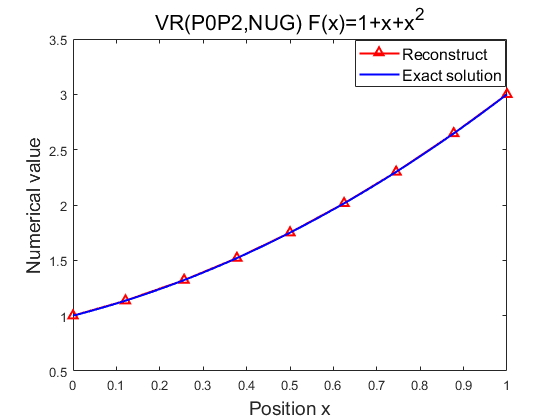
\includegraphics[width=3in]{P0P2VRreconstruct/Fu8.png} 
	}
	\hfill
	\subfloat[g重构]{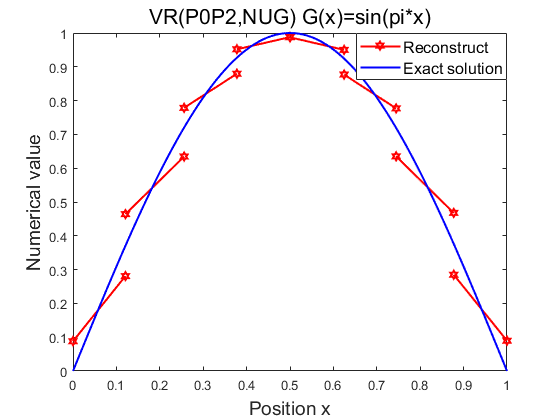
\includegraphics[width=3in]{P0P2VRreconstruct/Gu8.png} }
	\caption{VR P0P2重构(SGS(21))}
\end{figure}\leavevmode\\

	\begin{figure}[!h]
	\centering
	\subfloat[f精度分析]{
		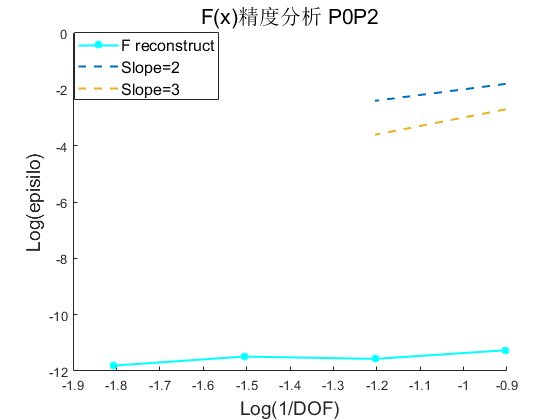
\includegraphics[width=3in]{P0P2VRreconstruct/F-1-1-1-omega0sqrt2.png} 
	}
	\hfill
	\subfloat[g精度分析]{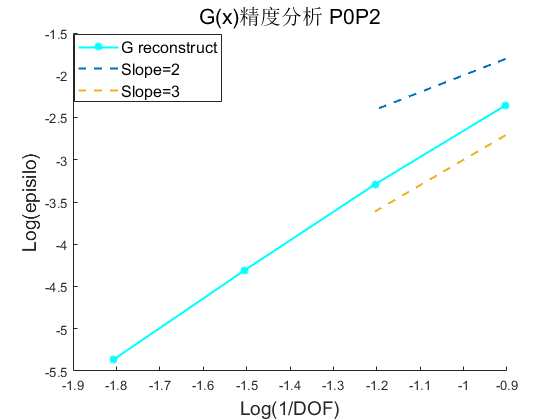
\includegraphics[width=3in]{P0P2VRreconstruct/G-1-1-1-omega0sqrt2.png} }
	\caption{VR P0P2精度分析}
\end{figure}\leavevmode\\
调整权重系数以及边界面权重系数,测试重构精度,得到以下结论:\\
	\begin{minipage}[c]{0.5\textwidth}
	\centering
	\label{tbl:table1}
	\captionof{table}{$F\left(x\right)$精度与$\omega_0$,$\omega_1$,$\omega_2$,$\omega_b$的关系} 
	\begin{tabular}{cccccc}
		\Xhline{2pt}
		\multirow{2}{*}{$\omega_0$} & \multirow{2}{*}{$\omega_1$}
		&\multirow{2}{*}{$\omega_2$}& \multirow{2}{*}{$\omega_b$}  & \multirow{2}{*}{精度表现}  \\
		\\
		\Xhline{0.5pt}\\
		0&—&—&—&差\\
		\Xhline{0.5pt}\\
		—&0&—&—&差\\
		\Xhline{0.5pt}\\
		—&—&0&—&差\\
		\Xhline{0.5pt}\\
		—&—&—& $\downarrow 1$&$\uparrow$ \\
		\Xhline{0.5pt}\\
		—&—&$\uparrow 1$&—&$\uparrow$\\
		\Xhline{0.5pt}\\
		—&$\uparrow 1$&—&—&$\uparrow$\\   
			\Xhline{0.5pt}\\
		$\uparrow 1$&—&—&—&$\uparrow$\\       
		\Xhline{2pt}
	\end{tabular}
\end{minipage}
\begin{minipage}[c]{0.5\textwidth}
	\centering
	\label{tbl:table1}
	\captionof{table}{$G\left(x\right)$精度与$\omega_0$,$\omega_1$,$\omega_2$,$\omega_b$的关系}  
	\begin{tabular}{cccccc}
		\Xhline{2pt}
		\multirow{2}{*}{$\omega_0$} & \multirow{2}{*}{$\omega_1$}&\multirow{2}{*}{$\omega_2$}& \multirow{2}{*}{$\omega_b$} & \multirow{2}{*}{精度表现}  \\
		\\
		\Xhline{0.5pt}\\
	0&—&—&—&差\\
	\Xhline{0.5pt}\\
	—&—&—& $\downarrow 1$&$\uparrow$ \\
	\Xhline{0.5pt}\\
	—&—&$\uparrow 0.5$&—&$\uparrow$\\
	\Xhline{0.5pt}\\
	—&$\uparrow 0.5$&—&—&$\uparrow$\\   
	\Xhline{0.5pt}\\
	$\uparrow 1$&—&—&—&$\uparrow$\\       
	\Xhline{2pt}
	\end{tabular}
\end{minipage}
\clearpage
 \textbf{解:P1P2}\\
 与P0P2类似,IJI的定义不变,但是限制方程组改变:\\
 \\$$\left\{
 \begin{aligned}
 	\frac{\partial I_f}{\partial u_{3L}}&=0\\
 	\frac{\partial I_f}{\partial u_{3R}}&=0
 \end{aligned}
 \right.$$\\
 该重构可用托马斯精确求解,下面展示权重$\omega_0=1, \omega_1=1, \omega_2=1, \omega_b=\frac{\omega_0}{\sqrt{2}}$, Nelem=8时的重构图和精度分析图:\\
 	\begin{figure}[!h]
 	\centering
 	\subfloat[f重构]{
 		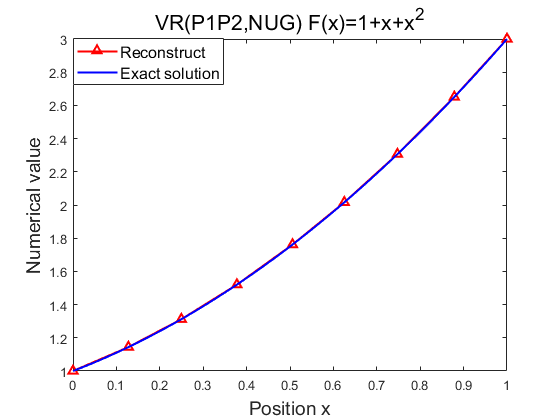
\includegraphics[width=3in]{P1P2VRreconstruct/Fu8.png} 
 	}
 	\hfill
 	\subfloat[g重构]{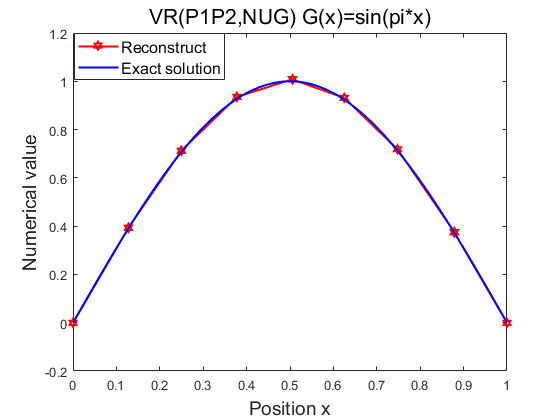
\includegraphics[width=3in]{P1P2VRreconstruct/Gu8.png} }
 	\caption{VR P1P2重构}
 \end{figure}\leavevmode\\
 
 \begin{figure}[!h]
 	\centering
 	\subfloat[f精度分析]{
 		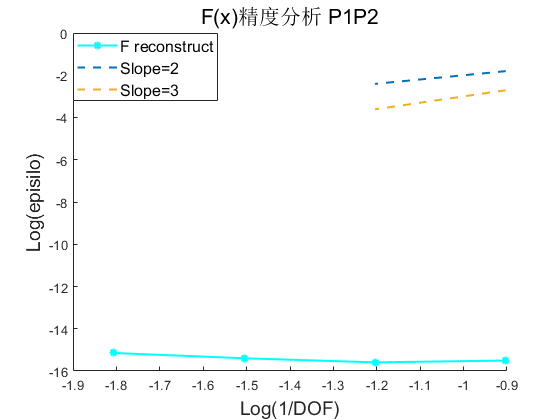
\includegraphics[width=3in]{P1P2VRreconstruct/F-1-1-1-omega0sqrt2.png} 
 	}
 	\hfill
 	\subfloat[g精度分析]{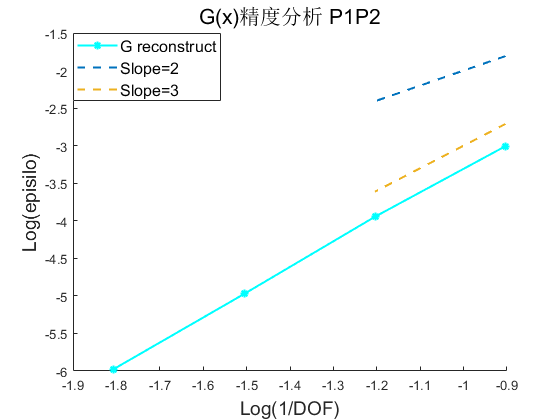
\includegraphics[width=3in]{P1P2VRreconstruct/G-1-1-1-omega0sqrt2.png} }
 	\caption{VR P1P2精度分析}
  \end{figure}\leavevmode\\
调整权重系数以及边界面权重系数,测试重构精度,得到以下结论:\\
~\\
\begin{minipage}[c]{0.5\textwidth}
	\centering
	\label{tbl:table1}
	\captionof{table}{$F\left(x\right)$精度与$\omega_0$,$\omega_1$,$\omega_2$,$\omega_b$的关系(P1P2)} 
	\begin{tabular}{cccccc}
		\Xhline{2pt}
		\multirow{2}{*}{$\omega_0$} & \multirow{2}{*}{$\omega_1$}
		&\multirow{2}{*}{$\omega_2$}& \multirow{2}{*}{$\omega_b$}  & \multirow{2}{*}{精度表现}  \\
		\\
		\Xhline{0.5pt}\\
		—&—&—& $\uparrow \frac{\omega_0}{\sqrt{2}}$&$\uparrow$ \\
		\Xhline{0.5pt}\\
		—&—&$\uparrow 1$&—&$\uparrow$\\
		\Xhline{0.5pt}\\
		—&$\uparrow 0.5$&—&—&$\uparrow$\\   
		\Xhline{0.5pt}\\
		改变&—&—&—&几乎无影响\\       
		\Xhline{2pt}
	\end{tabular}
\end{minipage}
\begin{minipage}[c]{0.5\textwidth}
	\centering
	\label{tbl:table1}
	\captionof{table}{$G\left(x\right)$精度与$\omega_0$,$\omega_1$,$\omega_2$,$\omega_b$的关系 (P1P2)}  
	\begin{tabular}{cccccc}
		\Xhline{2pt}
		\multirow{2}{*}{$\omega_0$} & \multirow{2}{*}{$\omega_1$}&\multirow{2}{*}{$\omega_2$}& \multirow{2}{*}{$\omega_b$} & \multirow{2}{*}{精度表现}  \\
		\\
		\Xhline{0.5pt}\\
		—&—&—& $\uparrow \frac{\omega_0}{\sqrt{2}}$&$\uparrow$ \\
		\Xhline{0.5pt}\\
		—&—&$\uparrow 1$&—&$\uparrow$\\
		\Xhline{0.5pt}\\
		—&$\uparrow 1$&—&—&$\uparrow$\\   
		\Xhline{0.5pt}\\
		改变&—&—&—&几乎无影响\\       
		\Xhline{2pt}
	\end{tabular}
\end{minipage}\leavevmode\\

\vspace{10em}
\noindent \textbf{b)解:}\\
考虑Hyperbolic rDG, 注意到\\
$$u=\begin{pmatrix}
	\varphi\\
	v
\end{pmatrix}=
\begin{pmatrix}
	B_1&B_2&B_3\\
	0&B_1\Delta x^{-1}& B_2 \Delta x^{-1}
\end{pmatrix}
\begin{pmatrix}
	\overline{\varphi}\\
	\overline{\varphi_x}\Delta x\\
	\varphi^{c,R}_{xx}\Delta x^2\\
\end{pmatrix}$$\\
$\Rightarrow$ $\left\{
\begin{aligned}
	\varphi_x&=v\\
	\varphi_{xx}&=v_x
\end{aligned}
\right.$ 所以,若$u_1=\overline{\varphi_i},u_2=\overline{\varphi_x}\Delta x_i, u_3=\varphi_{xx}^{c,R}\Delta X^2_I$,	则$\varphi=\sum_{i=1}^{3}u_iB_i$\\
$$I_f=\frac{1}{d_{LR}}\left(\omega^2_0\left[\varphi\right]^2+\omega^2_1\left[v\right]^2d^2_{LR}+\omega_2^2\left[v_{x}\right]^2d^4_{LR}\right)=\frac{1}{d_{LR}}\left(\omega^2_0\left[\varphi\right]^2+\omega^2_1\left[\varphi_x\right]^2d^2_{LR}+\omega_2^2\left[\varphi_{xx}\right]^2d^4_{LR}\right)$$\\
\indent 这与P1P2的VR是等价的,只不过$u_2$存储的量发生了改变。权重系数与边界系数对于重构精度的影响与P1P2的VR类似,这里不予展示。下面展示这种情况下权重$\omega_0=1, \omega_1=1, \omega_2=1, \omega_b=\frac{\omega_0}{\sqrt{2}}$, Nelem=8时的重构图和精度分析图:\\
	\begin{figure}[!h]
	\centering
	\subfloat[f重构]{
		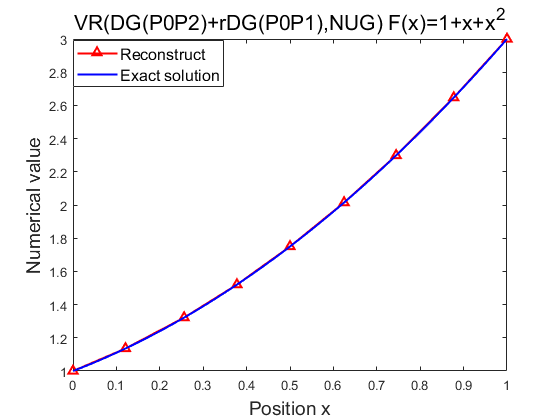
\includegraphics[width=3in]{Hyperbolic VR/Fu8.png} 
	}
	\hfill
	\subfloat[g重构]{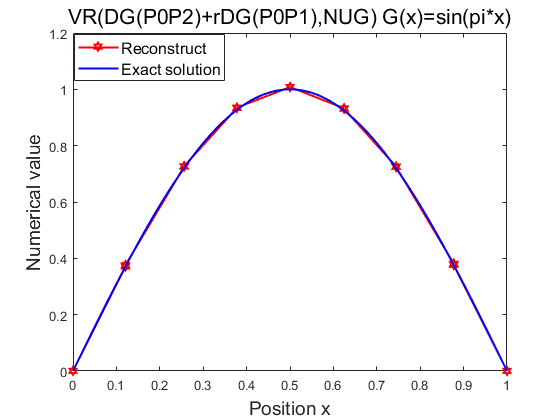
\includegraphics[width=3in]{Hyperbolic VR/Gu8.png} }
	\caption{VR DG(P0P2)+rDG(P0P1)}
\end{figure}\leavevmode\\

\begin{figure}[!h]
	\centering
	\subfloat[f精度分析]{
		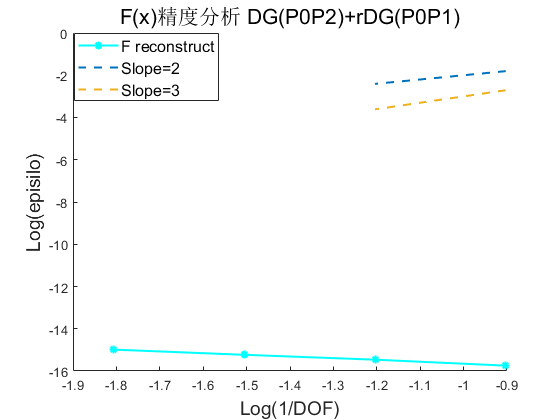
\includegraphics[width=3in]{Hyperbolic VR/F-1-1-1-omega0sqrt2.png} 
	}
	\hfill
	\subfloat[g精度分析]{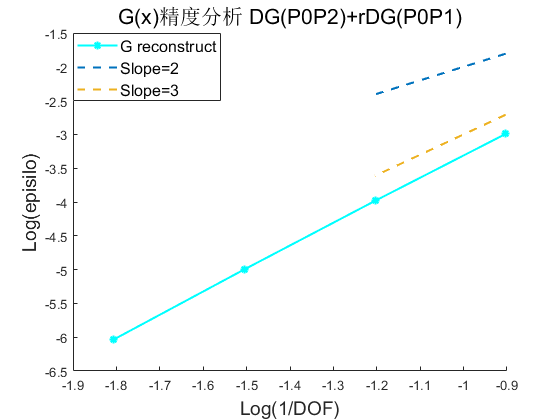
\includegraphics[width=3in]{Hyperbolic VR/G-1-1-1-omega0sqrt2.png} }
	\caption{VR DG(P0P2)+rDG(P0P1)精度分析}
\end{figure}
\clearpage
\section{附录}
\subsection{代码,仅展示部分}
\noindent \textbf{VRP0P2}
\lstset{language=Matlab}%代码语言使用的是matlab
\lstset{breaklines}%自动将长的代码行换行排版
\lstset{extendedchars=false}%解决代码跨页时,章节标题,页眉等汉字不显示的问题
\begin{lstlisting}
clc
clear all
close all
% Pre-proceeding
Unit=8;endx=1;deltax=endx/Unit;numberx=Unit+1;omega0=1;omega1=1;omega2=0.5;omegab=omega0/sqrt(2);
%记录内点位置,上下浮动不超过百分之5
Grid=zeros(1,numberx);
Deltax=zeros(1,Unit);
for i=2:numberx-1
Grid(1,i)=(i-1)*deltax+(0.1*rand(1)-0.05)*deltax;
end
Grid(1,numberx)=endx;
for i=2:numberx
Deltax(i-1)=Grid(1,i)-Grid(1,i-1);%记录每个单元的区间长度
end
f=@(x)1+x+x.^2;F=@(x)2.*x+1;
h=@(x)sin(pi*x);H=@(x)pi*cos(pi*x);
Unumsolution=zeros(1,Unit);
Ureconstruct=zeros(2*Unit,1);
A=sparse(1:2*Unit,1:2*Unit,0,2*Unit,2*Unit);
R=zeros(2*Unit,1);
Unumsolution1=zeros(1,2);
Unumsolution2=zeros(2,numberx-1);
Acc=zeros(3,4);a1=[1/8,1/16,1/32,1/64];a2=[1/8,1/16];

% Proceeding
%对f
%initial 
for i=1:numberx-1
Unumsolution(1,i)=(Grid(i+1)-Grid(i)+(Grid(i+1)^2-Grid(i)^2)/2+(Grid(i+1)^3-Grid(i)^3)/3)/(Grid(i+1)-Grid(i));
end

%构建大型分块稀疏矩阵
for iface=2:numberx-1
ieL=iface-1;xciL=0.5*(Grid(ieL)+Grid(ieL+1));
ieR=iface;xciR=0.5*(Grid(ieR)+Grid(ieR+1));
dLR=0.5*(Deltax(ieR)+Deltax(ieL));
B2L=(Grid(iface)-xciL)/Deltax(ieL);B2R=(Grid(iface)-xciR)/Deltax(ieR);
B3L=0.5*B2L^2-1/24;B3R=0.5*B2R^2-1/24;
%diag
A(2*ieL-1,2*ieL-1)=A(2*ieL-1,2*ieL-1)+2*(omega0^2*B2L^2+omega1^2*dLR^2/Deltax(ieL)^2)/dLR;
A(2*ieL-1,2*ieL)=A(2*ieL-1,2*ieL)+2*(omega0^2*B3L*B2L+omega1^2*dLR^2*B2L/Deltax(ieL)^2)/dLR;
A(2*ieL,2*ieL-1)=A(2*ieL,2*ieL-1)+2*(omega0^2*B2L*B3L+omega1^2*dLR^2*B2L/Deltax(ieL)^2)/dLR;
A(2*ieL,2*ieL)=A(2*ieL,2*ieL)+2*(omega0^2*B3L^2+omega1^2*dLR^2*B2L^2/Deltax(ieL)^2+omega2^2*dLR^4/Deltax(ieL)^4)/dLR;
A(2*ieR-1,2*ieR-1)=A(2*ieR-1,2*ieR-1)+2*(omega0^2*B2R^2+omega1^2*dLR^2/Deltax(ieR)^2)/dLR;
A(2*ieR-1,2*ieR)=A(2*ieR-1,2*ieR)+2*(omega0^2*B3R*B2R+omega1^2*dLR^2*B2R/Deltax(ieR)^2)/dLR;
A(2*ieR,2*ieR-1)=A(2*ieR,2*ieR-1)+2*(omega0^2*B2R*B3R+omega1^2*dLR^2*B2R/Deltax(ieR)^2)/dLR;
A(2*ieR,2*ieR)=A(2*ieR,2*ieR)+2*(omega0^2*B3R^2+omega1^2*dLR^2*B2R^2/Deltax(ieR)^2+omega2^2*dLR^4/Deltax(ieR)^4)/dLR;

%upper
A(2*ieL-1,2*ieR-1)=A(2*ieL-1,2*ieR-1)-2*(omega0^2*B2R*B2L+omega1^2*dLR^2/(Deltax(ieL)*Deltax(ieR)))/dLR;
A(2*ieL-1,2*ieR)=A(2*ieL-1,2*ieR)-2*(omega0^2*B3R*B2L+omega1^2*dLR^2*B2R/(Deltax(ieL)*Deltax(ieR)))/dLR;
A(2*ieL,2*ieR-1)=A(2*ieL,2*ieR-1)-2*(omega0^2*B2R*B3L+omega1^2*dLR^2*B2L/(Deltax(ieL)*Deltax(ieR)))/dLR;
A(2*ieL,2*ieR)=A(2*ieL,2*ieR)-2*(omega0^2*B3R*B3L+omega1^2*dLR^2*B2R*B2L/(Deltax(ieL)*Deltax(ieR))+omega2^2*dLR^4/(Deltax(ieL)^2*Deltax(ieR)^2))/dLR;
%lower
A(2*ieR-1,2*ieL-1)=A(2*ieR-1,2*ieL-1)-2*(omega0^2*B2L*B2R+omega1^2*dLR^2/(Deltax(ieL)*Deltax(ieR)))/dLR;
A(2*ieR-1,2*ieL)=A(2*ieR-1,2*ieL)-2*(omega0^2*B3L*B2R+omega1^2*dLR^2*B2L/(Deltax(ieR)*Deltax(ieL)))/dLR;
A(2*ieR,2*ieL-1)=A(2*ieR,2*ieL-1)-2*(omega0^2*B2L*B3R+omega1^2*dLR^2*B2R/(Deltax(ieR)*Deltax(ieL)))/dLR;
A(2*ieR,2*ieL)=A(2*ieR,2*ieL)-2*(omega0^2*B3L*B3R+omega1^2*dLR^2*B2L*B2R/(Deltax(ieR)*Deltax(ieL))+omega2^2*dLR^4/(Deltax(ieR)^2*Deltax(ieL)^2))/dLR;

%RHS
R(2*ieL-1)=R(2*ieL-1)-2*omega0^2*(Unumsolution(ieL)-Unumsolution(ieR))*B2L/dLR;
R(2*ieL)=R(2*ieL)-2*omega0^2*(Unumsolution(ieL)-Unumsolution(ieR))*B3L/dLR;
R(2*ieR-1)=R(2*ieR-1)+2*omega0^2*(Unumsolution(ieL)-Unumsolution(ieR))*B2R/dLR;
R(2*ieR)=R(2*ieR)+2*omega0^2*(Unumsolution(ieL)-Unumsolution(ieR))*B3R/dLR;    
end

%B.C
%left
iface=1;
ieR=iface;
xciR=0.5*(Grid(ieR)+Grid(ieR+1));
B2R=(Grid(iface)-xciR)/Deltax(ieR);
B3R=0.5*B2R^2-1/24;
A(2*ieR-1,2*ieR-1)=A(2*ieR-1,2*ieR-1)+4*omegab^2*B2R^2/Deltax(ieR);
A(2*ieR-1,2*ieR)=A(2*ieR-1,2*ieR)+4*omegab^2*B2R*B3R/Deltax(ieR);
A(2*ieR,2*ieR-1)=A(2*ieR,2*ieR-1)+4*omegab^2*B2R*B3R/Deltax(ieR);
A(2*ieR,2*ieR)=A(2*ieR,2*ieR)+4*omegab^2*B3R^2/Deltax(ieR);

R(2*ieR-1)=R(2*ieR-1)+4*omegab^2*(1-Unumsolution(ieR))*B2R/Deltax(ieR);
R(2*ieR)=R(2*ieR)+4*omegab^2*(1-Unumsolution(ieR))*B3R/Deltax(ieR);  

%Right
iface=numberx;
ieL=iface-1;
xciL=0.5*(Grid(ieL)+Grid(ieL+1));
B2L=(Grid(iface)-xciL)/Deltax(ieL);
B3L=0.5*B2L^2-1/24;

A(2*ieL-1,2*ieL-1)=A(2*ieL-1,2*ieL-1)+4*omegab^2*B2L^2/Deltax(ieL);
A(2*ieL-1,2*ieL)=A(2*ieL-1,2*ieL)+4*omegab^2*B2L*B3L/Deltax(ieL);
A(2*ieL,2*ieL-1)=A(2*ieL,2*ieL-1)+4*omegab^2*B2L*B3L/Deltax(ieL);
A(2*ieL,2*ieL)=A(2*ieL,2*ieL)+4*omegab^2*B3L^2/Deltax(ieL);

R(2*ieL-1)=R(2*ieL-1)-4*omegab^2*(Unumsolution(ieL)-3)*B2L/Deltax(ieL);
R(2*ieL)=R(2*ieL)-4*omegab^2*(Unumsolution(ieL)-3)*B3L/Deltax(ieL);



%LU-SGS 解三对角矩阵
%取出我们所需要的D
D=zeros(2*Unit,2*Unit);
for iface=2:numberx
ieL=iface-1;
D(2*ieL-1:2*ieL,2*ieL-1:2*ieL)=A(2*ieL-1:2*ieL,2*ieL-1:2*ieL);
end
%取出我们所需要的L
L=zeros(2*Unit,2*Unit);
for iface=2:numberx-1
ieR=iface;
ieL=iface-1;
L(2*ieR-1:2*ieR,2*ieL-1:2*ieL)=A(2*ieR-1:2*ieR,2*ieL-1:2*ieL);
end

%取出我们所需要的U
U=zeros(2*Unit,2*Unit);
for iface=2:numberx-1
ieR=iface;
ieL=iface-1;
U(2*ieL-1:2*ieL,2*ieR-1:2*ieR)= A(2*ieL-1:2*ieL,2*ieR-1:2*ieR);
end
b=R;%用来存储最初的rhs
Ureconstruct0=zeros(2*Unit,1);
for k=1:30%k表示SGS(k)
%Forward sweep
ie=1;
Ureconstruct(ie:ie+1,1)=D(ie:ie+1,ie:ie+1)\R(ie:ie+1,1);
for ie=2:numberx-1
R(2*ie-1:2*ie,1)=R(2*ie-1:2*ie,1)-L(2*ie-1:2*ie,2*(ie-1)-1:2*(ie-1))*Ureconstruct(2*(ie-1)-1:2*(ie-1),1);
Ureconstruct(2*ie-1:2*ie,1)=D(2*ie-1:2*ie,2*ie-1:2*ie)\R(2*ie-1:2*ie,1);
end
%Backward sweep
for ie=1:numberx-1
R(2*ie-1:2*ie,1)= D(2*ie-1:2*ie,2*ie-1:2*ie)*Ureconstruct(2*ie-1:2*ie,1);
end

ie=numberx-1;
Ureconstruct(2*ie-1:2*ie)=D(2*ie-1:2*ie,2*ie-1:2*ie)\R(2*ie-1:2*ie,1);
for ie=numberx-2:-1:1
R(2*ie-1:2*ie,1)=R(2*ie-1:2*ie,1)-U(2*ie-1:2*ie,2*(ie+1)-1:2*(ie+1))*Ureconstruct(2*(ie+1)-1:2*(ie+1),1);
Ureconstruct(2*ie-1:2*ie,1)=D(2*ie-1:2*ie,2*ie-1:2*ie)\R(2*ie-1:2*ie,1);
end
deltaUreconstruct=Ureconstruct;
Ureconstruct=Ureconstruct0+Ureconstruct;
if max(deltaUreconstruct)<10^(-10)
break;
end
%重新整理R
R=b-A*Ureconstruct;
Ureconstruct0=Ureconstruct;
end  
% Post-proceeding
figure
k=1;
x=Grid(k):1*(Grid(k+1)-Grid(k)):Grid(k+1);
xci=(Grid(k+1)+Grid(k))/2;
p=@(x)Unumsolution(1,k)+Ureconstruct(2*k-1,1)*(x-xci)/Deltax(k)+Ureconstruct(2*k,1)*(0.5*((x-xci)/Deltax(k)).^2-1/24);
y=p(x);
plot(x,y,'-r^','linewidth',1.5);hold on
H1=plot(x,y,'-r^','linewidth',1.5);hold on

for k=2:numberx-1
x=Grid(k):1*(Grid(k+1)-Grid(k)):Grid(k+1);
xci=(Grid(k+1)+Grid(k))/2;
p=@(x)Unumsolution(1,k)+Ureconstruct(2*k-1,1)*(x-xci)/Deltax(k)+Ureconstruct(2*k,1)*(0.5*((x-xci)/Deltax(k)).^2-1/24);
y=p(x);
plot(x,y,'-r^','linewidth',1.5);
end

hold on
x=Grid(1):0.01*(Grid(numberx)-Grid(1)):Grid(numberx);
plot(x,f(x),'-b','linewidth',1.5);
H2=plot(x,f(x),'-b','linewidth',1.5);
lgd=legend([H1,H2],'Reconstruct','Exact solution');
lgd.FontSize=12;
xlabel('Position x','fontsize',14)
ylabel('Numerical value','fontsize',14)
title('VR(P0P2,NUG) F(x)=1+x+x^2','fontsize',16)
hold off

%计算精度
Acc(1,1)=Accuracy(8);
Acc(1,2)=Accuracy(16);
Acc(1,3)=Accuracy(32);
Acc(1,4)=Accuracy(64);
for k=1:3
accuracyf(k)=(log10(Acc(1,k+1))-log10(Acc(1,k)))./(log10(a1(1,k+1))-log10(a1(1,k)));
end

figure
hold on
plot(log10(a1),log10(Acc(1,:)),'-c*','linewidth',1.5)
H1=plot(log10(a1),log10(Acc(1,:)),'-c*','linewidth',1.5);

H2=plot(log10(a2),2*log10(a2),'--','linewidth',1.5);
plot(log10(a2),3*log10(a2),'--','linewidth',1.5)
H3=plot(log10(a2),3*log10(a2),'--','linewidth',1.5);
lgd=legend([H1,H2,H3],'F reconstruct','Slope=2','Slope=3');
lgd.FontSize=12;
xlabel('Log(1/DOF)','fontsize',14)
ylabel('Log(episilo)','fontsize',14)
title('F(x)精度分析 P0P2','fontsize',16)
\end{lstlisting}

	\subsection{部分精度比较图}
	\begin{figure}[!h]
		\centering
		\subfloat[$\omega_0=1,\omega_1=1,\omega_2=1,\omega_b=\frac{\omega_0}{\sqrt{2}}$]{
			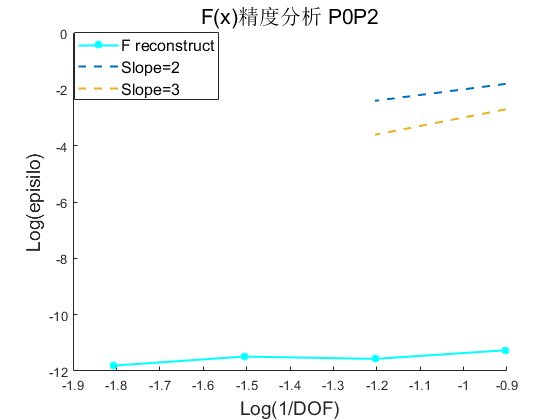
\includegraphics[width=2.5in]{P0P2VRreconstruct/F-1-1-1-omega0sqrt2.png} 
		}
		\hfill
		\subfloat[$\omega_0=1,\omega_1=1,\omega_2=1,\omega_b=\frac{\omega_0}{\sqrt{2}}$]{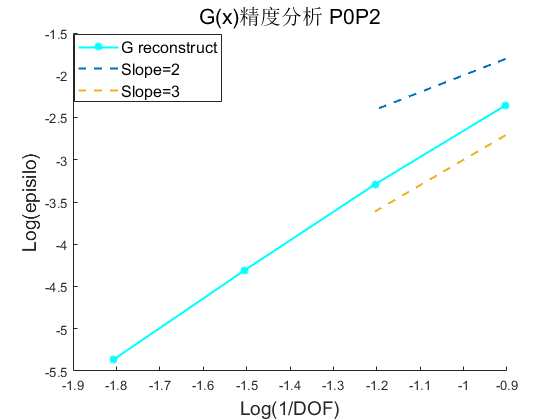
\includegraphics[width=2.5in]{P0P2VRreconstruct/G-1-1-1-omega0sqrt2.png} }\\
		\subfloat[$\omega_0=1,\omega_1=1,\omega_2=1,\omega_b=1$]{
			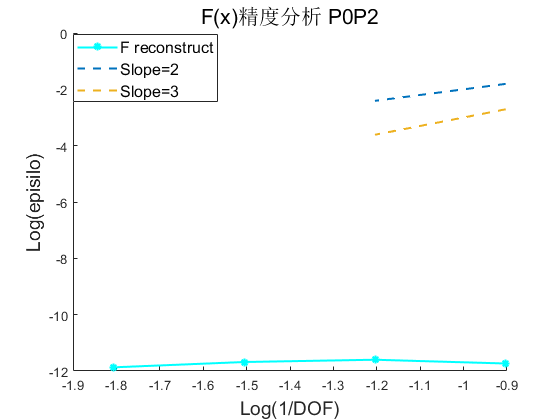
\includegraphics[width=2.5in]{P0P2VRreconstruct/F-1-1-1-1.png} 
		}
		\hfill
		\subfloat[$\omega_0=1,\omega_1=1,\omega_2=1,\omega_b=1$]{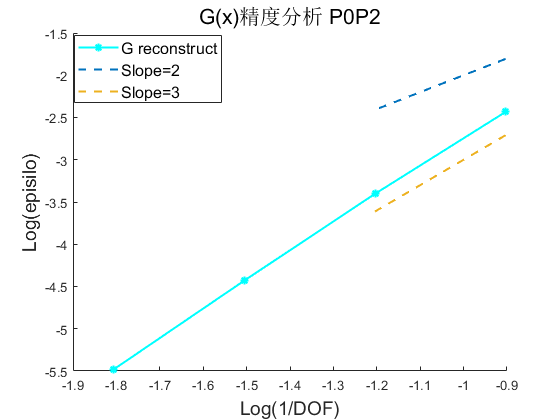
\includegraphics[width=2.5in]{P0P2VRreconstruct/G-1-1-1-1.png} }\\
		\subfloat[$\omega_0=1,\omega_1=1,\omega_2=0,\omega_b=\frac{\omega_0}{\sqrt{2}}$]{
			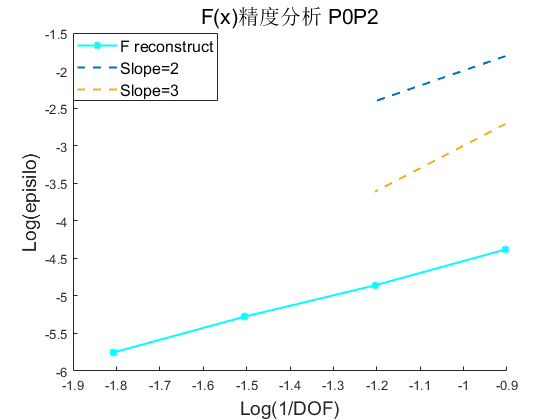
\includegraphics[width=2.5in]{P0P2VRreconstruct/F-1-1-0-omega0sqrt2.png} 
		}
		\hfill
		\subfloat[$\omega_0=1,\omega_1=1,\omega_2=0,\omega_b=\frac{\omega_0}{\sqrt{2}}$]{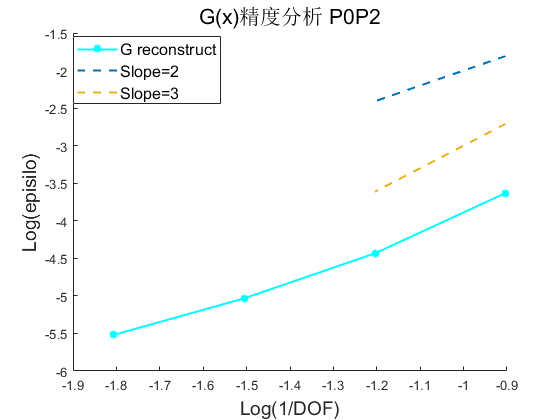
\includegraphics[width=2.5in]{P0P2VRreconstruct/G-1-1-0-omega0sqrt2.png} }\\
		\subfloat[$\omega_0=1,\omega_1=1,\omega_2=0.5,\omega_b=\frac{\omega_0}{\sqrt{2}}$]{
			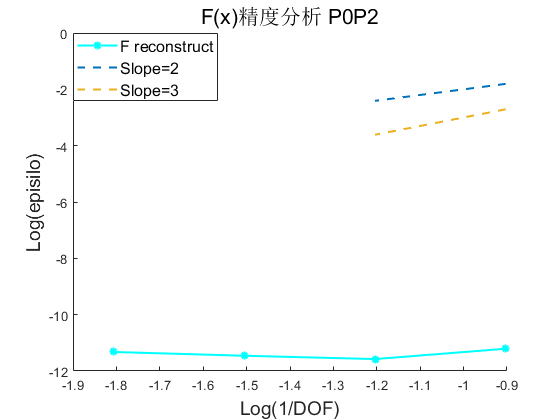
\includegraphics[width=2.5in]{P0P2VRreconstruct/F-1-1-0.5-omega0sqrt2.png} 
		}
		\hfill
		\subfloat[$\omega_0=1,\omega_1=1,\omega_2=0.5,\omega_b=\frac{\omega_0}{\sqrt{2}}$]{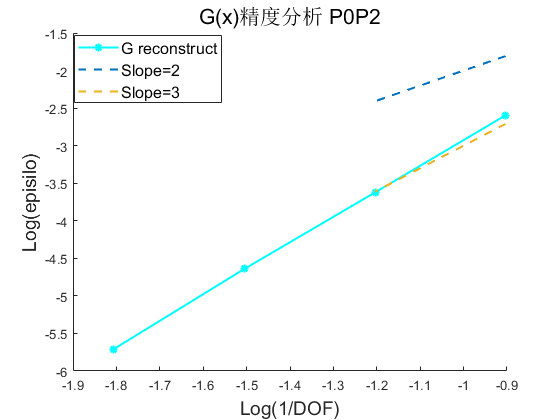
\includegraphics[width=2.5in]{P0P2VRreconstruct/G-1-1-0.5-omega0sqrt2.png} }		
		\caption{VR精度分析(P0P2调整权重系数)}
	\end{figure}
	\begin{figure}[!h]
	\centering
	\subfloat[$\omega_0=1,\omega_1=1,\omega_2=1,\omega_b=\frac{\omega_0}{\sqrt{2}}$]{
		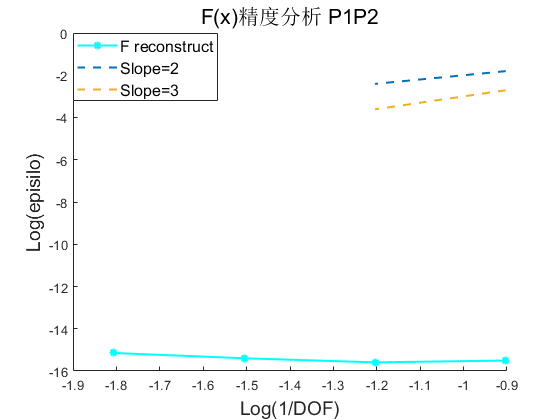
\includegraphics[width=2.5in]{P1P2VRreconstruct/F-1-1-1-omega0sqrt2.png} 
	}
	\hfill
	\subfloat[$\omega_0=1,\omega_1=1,\omega_2=1,\omega_b=\frac{\omega_0}{\sqrt{2}}$]{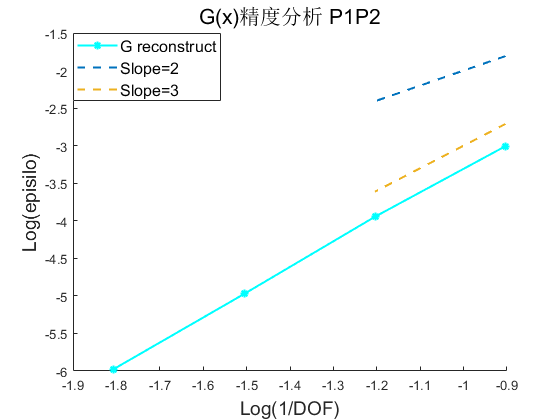
\includegraphics[width=2.5in]{P1P2VRreconstruct/G-1-1-1-omega0sqrt2.png} }\\
	\subfloat[$\omega_0=1,\omega_1=1,\omega_2=1,\omega_b=1$]{
		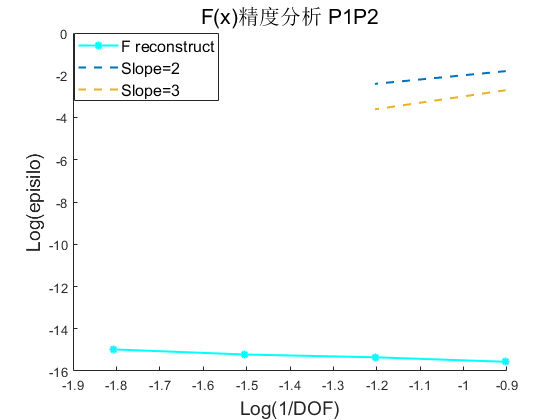
\includegraphics[width=2.5in]{P1P2VRreconstruct/F-1-1-1-1.png} 
	}
	\hfill
	\subfloat[$\omega_0=1,\omega_1=1,\omega_2=1,\omega_b=1$]{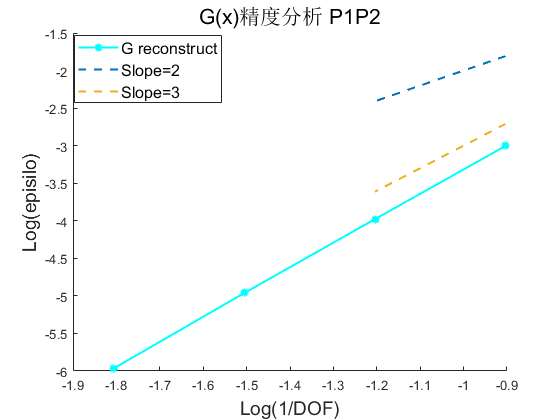
\includegraphics[width=2.5in]{P1P2VRreconstruct/G-1-1-1-1.png} }\\
	\subfloat[$\omega_0=1,\omega_1=1,\omega_2=0,\omega_b=\frac{\omega_0}{\sqrt{2}}$]{
		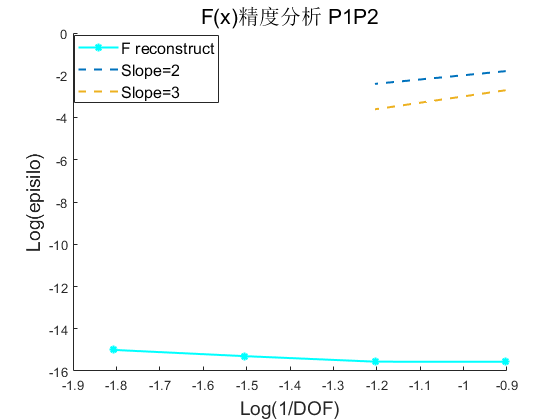
\includegraphics[width=2.5in]{P1P2VRreconstruct/F-1-1-0-omega0sqrt2.png} 
	}
	\hfill
	\subfloat[$\omega_0=1,\omega_1=1,\omega_2=0,\omega_b=\frac{\omega_0}{\sqrt{2}}$]{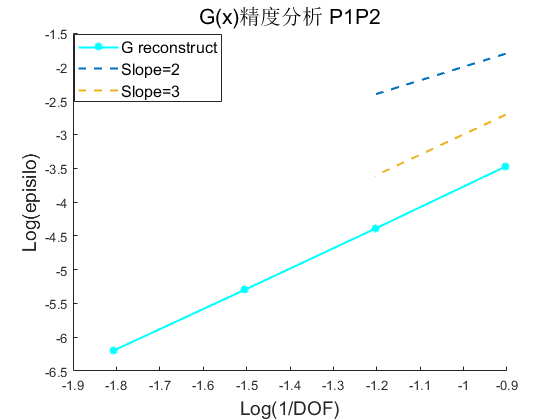
\includegraphics[width=2.5in]{P1P2VRreconstruct/G-1-1-0-omega0sqrt2.png} }\\
	\subfloat[$\omega_0=1,\omega_1=1,\omega_2=0.5,\omega_b=\frac{\omega_0}{\sqrt{2}}$]{
		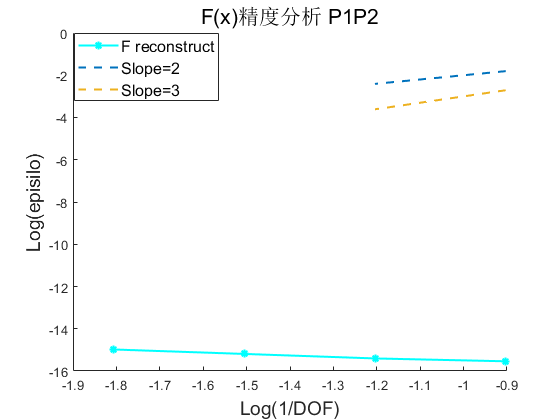
\includegraphics[width=2.5in]{P1P2VRreconstruct/F-1-1-0.5-omega0sqrt2.png} 
	}
	\hfill
	\subfloat[$\omega_0=1,\omega_1=1,\omega_2=0.5,\omega_b=\frac{\omega_0}{\sqrt{2}}$]{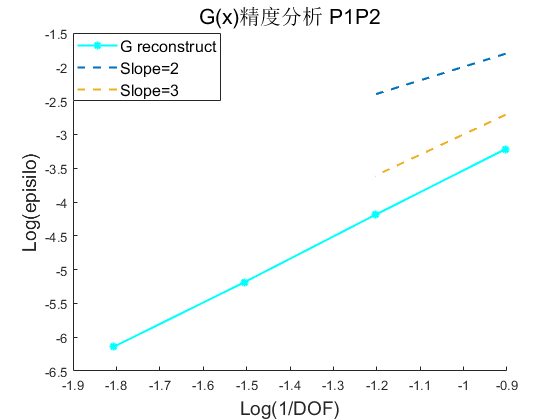
\includegraphics[width=2.5in]{P1P2VRreconstruct/G-1-1-0.5-omega0sqrt2.png} }		
	\caption{VR精度分析(P1P2调整权重系数)}
\end{figure}

	
		
\end{document}